191. Обозначим буквами отрезки на картинке.
\begin{center}
\begin{figure}[ht!]
\center{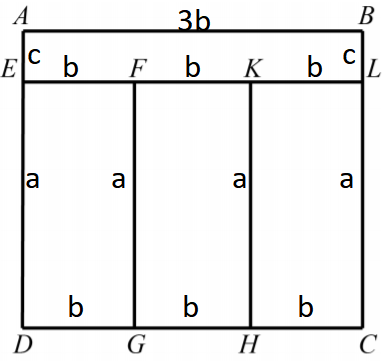
\includegraphics[scale=0.35]{41s.png}}
\end{figure}
\end{center}
Стороны, обозначенные буквой $a$ у прямоугольников одинаковые, периметры тоже, а поэтому одинаковы и стороны, обозначенные буквой $b.$ Тогда $3b=18,\ b=6$ см. Так как периметры одинаковы, имеем равенство $2\cdot(c+18)=2\cdot(6+a),\ c+18=6+16-c,\ 2c+18=22,\ c=2$см. Тогда у прямоугольника $ABLE$ стороны равны 2см и 18см, а у остальных прямоугольников --- 6см и $16-2=14$см.\\
